%%%%%%%%%%%%%%%%%%%%%%%%%%%%%%%%%%%%%%%%%
%  My documentation report
%  Objetive: Explain what I did and how, so someone can continue with the investigation
%
% Important note:
% Chapter heading images should have a 2:1 width:height ratio,
% e.g. 920px width and 460px height.
%
%%%%%%%%%%%%%%%%%%%%%%%%%%%%%%%%%%%%%%%%%

%----------------------------------------------------------------------------------------
%	PACKAGES AND OTHER DOCUMENT CONFIGURATIONS
%----------------------------------------------------------------------------------------

\documentclass[12pt,fleqn]{report} % Default font size and left-justified equations

\usepackage[top=3cm,bottom=3cm,left=3.2cm,right=3.2cm,headsep=10pt,letterpaper]{geometry} % Page margins

\usepackage{xcolor} % Required for specifying colors by name
\definecolor{ocre}{RGB}{243,102,25} % Define the orange color used for highlighting throughout the book

% Font Settings
\usepackage{avant} % Use the Avantgarde font for headings
%\usepackage{times} % Use the Times font for headings
\usepackage{mathptmx} % Use the Adobe Times Roman as the default text font together with math symbols from the Sym­bol, Chancery and Com­puter Modern fonts

\usepackage{microtype} % Slightly tweak font spacing for aesthetics
\usepackage[utf8]{inputenc} % Required for including letters with accents
\usepackage[T1]{fontenc} % Use 8-bit encoding that has 256 glyphs

% Bibliography
\usepackage[style=alphabetic,sorting=nyt,sortcites=true,autopunct=true,babel=hyphen,hyperref=true,abbreviate=false,backref=true,backend=biber]{biblatex}
\addbibresource{bibliography.bib} % BibTeX bibliography file
\defbibheading{bibempty}{}

%----------------------------------------------------------------------------------------
%	VARIOUS REQUIRED PACKAGES
%----------------------------------------------------------------------------------------

\usepackage{titlesec} % Allows customization of titles

\usepackage{graphicx} % Required for including pictures
\graphicspath{{Pictures/}} % Specifies the directory where pictures are stored

\usepackage{lipsum} % Inserts dummy text

\usepackage{tikz} % Required for drawing custom shapes

\usepackage[english]{babel} % English language/hyphenation

\usepackage{enumitem} % Customize lists
\setlist{nolistsep} % Reduce spacing between bullet points and numbered lists

\usepackage{booktabs} % Required for nicer horizontal rules in tables

\usepackage{eso-pic} % Required for specifying an image background in the title page

%----------------------------------------------------------------------------------------
%	MAIN TABLE OF CONTENTS
%----------------------------------------------------------------------------------------

\usepackage{titletoc} % Required for manipulating the table of contents

\contentsmargin{0cm} % Removes the default margin
% Chapter text styling
\titlecontents{chapter}[1.25cm] % Indentation
{\addvspace{15pt}\large\sffamily\bfseries} % Spacing and font options for chapters
{\color{ocre!60}\contentslabel[\Large\thecontentslabel]{1.25cm}\color{ocre}} % Chapter number
{}  
{\color{ocre!60}\normalsize\sffamily\bfseries\;\titlerule*[.5pc]{.}\;\thecontentspage} % Page number
% Section text styling
\titlecontents{section}[1.25cm] % Indentation
{\addvspace{5pt}\sffamily\bfseries} % Spacing and font options for sections
{\contentslabel[\thecontentslabel]{1.25cm}} % Section number
{}
{\sffamily\hfill\color{black}\thecontentspage} % Page number
[]
% Subsection text styling
\titlecontents{subsection}[1.25cm] % Indentation
{\addvspace{1pt}\sffamily\small} % Spacing and font options for subsections
{\contentslabel[\thecontentslabel]{1.25cm}} % Subsection number
{}
{\sffamily\;\titlerule*[.5pc]{.}\;\thecontentspage} % Page number
[] 

%----------------------------------------------------------------------------------------
%	MINI TABLE OF CONTENTS IN CHAPTER HEADS
%----------------------------------------------------------------------------------------

% Section text styling
\titlecontents{lsection}[0em] % Indendating
{\footnotesize\sffamily} % Font settings
{}
{}
{}

% Subsection text styling
\titlecontents{lsubsection}[.5em] % Indentation
{\normalfont\footnotesize\sffamily} % Font settings
{}
{}
{}
 
%----------------------------------------------------------------------------------------
%	PAGE HEADERS
%----------------------------------------------------------------------------------------

\usepackage{fancyhdr} % Required for header and footer configuration

\pagestyle{fancy}
\renewcommand{\chaptermark}[1]{\markboth{\sffamily\normalsize\bfseries\chaptername\ \thechapter.\ #1}{}} % Chapter text font settings
\renewcommand{\sectionmark}[1]{\markright{\sffamily\normalsize\thesection\hspace{5pt}#1}{}} % Section text font settings
\fancyhf{} \fancyhead[LE,RO]{\sffamily\normalsize\thepage} % Font setting for the page number in the header
\fancyhead[LO]{\rightmark} % Print the nearest section name on the left side of odd pages
\fancyhead[RE]{\leftmark} % Print the current chapter name on the right side of even pages
\renewcommand{\headrulewidth}{0.5pt} % Width of the rule under the header
\addtolength{\headheight}{2.5pt} % Increase the spacing around the header slightly
\renewcommand{\footrulewidth}{0pt} % Removes the rule in the footer
\fancypagestyle{plain}{\fancyhead{}\renewcommand{\headrulewidth}{0pt}} % Style for when a plain pagestyle is specified

% Removes the header from odd empty pages at the end of chapters
\makeatletter
\renewcommand{\cleardoublepage}{
\clearpage\ifodd\c@page\else
\hbox{}
\vspace*{\fill}
\thispagestyle{empty}
\newpage
\fi}

%----------------------------------------------------------------------------------------
%	THEOREM STYLES
%----------------------------------------------------------------------------------------

\usepackage{amsmath,amsfonts,amssymb,amsthm} % For math equations, theorems, symbols, etc

\newcommand{\intoo}[2]{\mathopen{]}#1\,;#2\mathclose{[}}
\newcommand{\ud}{\mathop{\mathrm{{}d}}\mathopen{}}
\newcommand{\intff}[2]{\mathopen{[}#1\,;#2\mathclose{]}}
\newtheorem{notation}{Notation}[chapter]

%%%%%%%%%%%%%%%%%%%%%%%%%%%%%%%%%%%%%%%%%%%%%%%%%%%%%%%%%%%%%%%%%%%%%%%%%%%
%%%%%%%%%%%%%%%%%%%% dedicated to boxed/framed environements %%%%%%%%%%%%%%
%%%%%%%%%%%%%%%%%%%%%%%%%%%%%%%%%%%%%%%%%%%%%%%%%%%%%%%%%%%%%%%%%%%%%%%%%%%
\newtheoremstyle{ocrenumbox}% % Theorem style name
{0pt}% Space above
{0pt}% Space below
{\normalfont}% % Body font
{}% Indent amount
{\small\bf\sffamily\color{ocre}}% % Theorem head font
{\;}% Punctuation after theorem head
{0.25em}% Space after theorem head
{\small\sffamily\color{ocre}\thmname{#1}\nobreakspace\thmnumber{\@ifnotempty{#1}{}\@upn{#2}}% Theorem text (e.g. Theorem 2.1)
\thmnote{\nobreakspace\the\thm@notefont\sffamily\bfseries\color{black}---\nobreakspace#3.}} % Optional theorem note
\renewcommand{\qedsymbol}{$\blacksquare$}% Optional qed square

\newtheoremstyle{blacknumex}% Theorem style name
{5pt}% Space above
{5pt}% Space below
{\normalfont}% Body font
{} % Indent amount
{\small\bf\sffamily}% Theorem head font
{\;}% Punctuation after theorem head
{0.25em}% Space after theorem head
{\small\sffamily{\tiny\ensuremath{\blacksquare}}\nobreakspace\thmname{#1}\nobreakspace\thmnumber{\@ifnotempty{#1}{}\@upn{#2}}% Theorem text (e.g. Theorem 2.1)
\thmnote{\nobreakspace\the\thm@notefont\sffamily\bfseries---\nobreakspace#3.}}% Optional theorem note

\newtheoremstyle{blacknumbox} % Theorem style name
{0pt}% Space above
{0pt}% Space below
{\normalfont}% Body font
{}% Indent amount
{\small\bf\sffamily}% Theorem head font
{\;}% Punctuation after theorem head
{0.25em}% Space after theorem head
{\small\sffamily\thmname{#1}\nobreakspace\thmnumber{\@ifnotempty{#1}{}\@upn{#2}}% Theorem text (e.g. Theorem 2.1)
\thmnote{\nobreakspace\the\thm@notefont\sffamily\bfseries---\nobreakspace#3.}}% Optional theorem note

%%%%%%%%%%%%%%%%%%%%%%%%%%%%%%%%%%%%%%%%%%%%%%%%%%%%%%%%%%%%%%%%%%%%%%%%%%%
%%%%%%%%%%%%% dedicated to non-boxed/non-framed environements %%%%%%%%%%%%%
%%%%%%%%%%%%%%%%%%%%%%%%%%%%%%%%%%%%%%%%%%%%%%%%%%%%%%%%%%%%%%%%%%%%%%%%%%%
\newtheoremstyle{ocrenum}% % Theorem style name
{5pt}% Space above
{5pt}% Space below
{\normalfont}% % Body font
{}% Indent amount
{\small\bf\sffamily\color{ocre}}% % Theorem head font
{\;}% Punctuation after theorem head
{0.25em}% Space after theorem head
{\small\sffamily\color{ocre}\thmname{#1}\nobreakspace\thmnumber{\@ifnotempty{#1}{}\@upn{#2}}% Theorem text (e.g. Theorem 2.1)
\thmnote{\nobreakspace\the\thm@notefont\sffamily\bfseries\color{black}---\nobreakspace#3.}} % Optional theorem note
\renewcommand{\qedsymbol}{$\blacksquare$}% Optional qed square
\makeatother

% Defines the theorem text style for each type of theorem to one of the three styles above
\newcounter{dummy} 
\numberwithin{dummy}{section}
\theoremstyle{ocrenumbox}
\newtheorem{theoremeT}[dummy]{Theorem}
\newtheorem{problem}{Problem}[chapter]
\newtheorem{exerciseT}{Exercise}[chapter]
\theoremstyle{blacknumex}
\newtheorem{exampleT}{Example}[chapter]
\theoremstyle{blacknumbox}
\newtheorem{vocabulary}{Vocabulary}[chapter]
\newtheorem{definitionT}{Definition}[section]
\newtheorem{corollaryT}[dummy]{Corollary}
\theoremstyle{ocrenum}
\newtheorem{proposition}[dummy]{Proposition}

%----------------------------------------------------------------------------------------
%	DEFINITION OF COLORED BOXES
%----------------------------------------------------------------------------------------

\RequirePackage[framemethod=default]{mdframed} % Required for creating the theorem, definition, exercise and corollary boxes

% Theorem box
\newmdenv[skipabove=7pt,
skipbelow=7pt,
backgroundcolor=black!5,
linecolor=ocre,
innerleftmargin=5pt,
innerrightmargin=5pt,
innertopmargin=5pt,
leftmargin=0cm,
rightmargin=0cm,
innerbottommargin=5pt]{tBox}

% Exercise box	  
\newmdenv[skipabove=7pt,
skipbelow=7pt,
rightline=false,
leftline=true,
topline=false,
bottomline=false,
backgroundcolor=ocre!10,
linecolor=ocre,
innerleftmargin=5pt,
innerrightmargin=5pt,
innertopmargin=5pt,
innerbottommargin=5pt,
leftmargin=0cm,
rightmargin=0cm,
linewidth=4pt]{eBox}	

% Definition box
\newmdenv[skipabove=7pt,
skipbelow=7pt,
rightline=false,
leftline=true,
topline=false,
bottomline=false,
linecolor=ocre,
innerleftmargin=5pt,
innerrightmargin=5pt,
innertopmargin=0pt,
leftmargin=0cm,
rightmargin=0cm,
linewidth=4pt,
innerbottommargin=0pt]{dBox}	

% Corollary box
\newmdenv[skipabove=7pt,
skipbelow=7pt,
rightline=false,
leftline=true,
topline=false,
bottomline=false,
linecolor=gray,
backgroundcolor=black!5,
innerleftmargin=5pt,
innerrightmargin=5pt,
innertopmargin=5pt,
leftmargin=0cm,
rightmargin=0cm,
linewidth=4pt,
innerbottommargin=5pt]{cBox}

% Creates an environment for each type of theorem and assigns it a theorem text style from the "Theorem Styles" section above and a colored box from above
\newenvironment{theorem}{\begin{tBox}\begin{theoremeT}}{\end{theoremeT}\end{tBox}}
\newenvironment{exercise}{\begin{eBox}\begin{exerciseT}}{\hfill{\color{ocre}\tiny\ensuremath{\blacksquare}}\end{exerciseT}\end{eBox}}				  
\newenvironment{definition}{\begin{dBox}\begin{definitionT}}{\end{definitionT}\end{dBox}}	
\newenvironment{example}{\begin{exampleT}}{\hfill{\tiny\ensuremath{\blacksquare}}\end{exampleT}}		
\newenvironment{corollary}{\begin{cBox}\begin{corollaryT}}{\end{corollaryT}\end{cBox}}	

%----------------------------------------------------------------------------------------
%	REMARK ENVIRONMENT
%----------------------------------------------------------------------------------------

\newenvironment{remark}{\par\vspace{10pt}\small % Vertical white space above the remark and smaller font size
\begin{list}{}{
\leftmargin=35pt % Indentation on the left
\rightmargin=25pt}\item\ignorespaces % Indentation on the right
\makebox[-2.5pt]{\begin{tikzpicture}[overlay]
\node[draw=ocre!60,line width=1pt,circle,fill=ocre!25,font=\sffamily\bfseries,inner sep=2pt,outer sep=0pt] at (-15pt,0pt){\textcolor{ocre}{R}};\end{tikzpicture}} % Orange R in a circle
\advance\baselineskip -1pt}{\end{list}\vskip5pt} % Tighter line spacing and white space after remark

%----------------------------------------------------------------------------------------
%	SECTION NUMBERING IN THE MARGIN
%----------------------------------------------------------------------------------------

\makeatletter
\renewcommand{\@seccntformat}[1]{\llap{\textcolor{ocre}{\csname the#1\endcsname}\hspace{1em}}}                    
\renewcommand{\section}{\@startsection{section}{1}{\z@}
{-4ex \@plus -1ex \@minus -.4ex}
{1ex \@plus.2ex }
{\normalfont\large\sffamily\bfseries}}
\renewcommand{\subsection}{\@startsection {subsection}{2}{\z@}
{-3ex \@plus -0.1ex \@minus -.4ex}
{0.5ex \@plus.2ex }
{\normalfont\sffamily\bfseries}}
\renewcommand{\subsubsection}{\@startsection {subsubsection}{3}{\z@}
{-2ex \@plus -0.1ex \@minus -.2ex}
{.2ex \@plus.2ex }
{\normalfont\small\sffamily\bfseries}}                        
\renewcommand\paragraph{\@startsection{paragraph}{4}{\z@}
{-2ex \@plus-.2ex \@minus .2ex}
{.1ex}
{\normalfont\small\sffamily\bfseries}}

%----------------------------------------------------------------------------------------
%	HYPERLINKS IN THE DOCUMENTS
%----------------------------------------------------------------------------------------

% For an unclear reason, the package should be loaded now and not later
\usepackage{hyperref}
\hypersetup{hidelinks,backref=true,pagebackref=true,hyperindex=true,colorlinks=false,breaklinks=true,urlcolor= ocre,bookmarks=true,bookmarksopen=false,pdftitle={Title},pdfauthor={Author}}

%----------------------------------------------------------------------------------------
%	CHAPTER HEADINGS
%----------------------------------------------------------------------------------------

% The set-up below should be (sadly) manually adapted to the overall margin page septup controlled by the geometry package loaded in the main.tex document. It is possible to implement below the dimensions used in the goemetry package (top,bottom,left,right)... TO BE DONE

\newcommand{\thechapterimage}{}
\newcommand{\chapterimage}[1]{\renewcommand{\thechapterimage}{#1}}

% Numbered chapters with mini tableofcontents
\def\thechapter{\arabic{chapter}}
\def\@makechapterhead#1{
\thispagestyle{empty}
{\centering \normalfont\sffamily
\ifnum \c@secnumdepth >\m@ne
\if@mainmatter
\startcontents
\begin{tikzpicture}[remember picture,overlay]
\node at (current page.north west)
{\begin{tikzpicture}[remember picture,overlay]
\node[anchor=north west,inner sep=0pt] at (0,0) {\includegraphics[width=\paperwidth]{\thechapterimage}};
%%%%%%%%%%%%%%%%%%%%%%%%%%%%%%%%%%%%%%%%%%%%%%%%%%%%%%%%%%%%%%%%%%%%%%%%%%%%%%%%%%%%%
% Commenting the 3 lines below removes the small contents box in the chapter heading
%\fill[color=ocre!10!white,opacity=.6] (1cm,0) rectangle (8cm,-7cm);
%\node[anchor=north west] at (1.1cm,.35cm) {\parbox[t][8cm][t]{6.5cm}{\huge\bfseries\flushleft \printcontents{l}{1}{\setcounter{tocdepth}{2}}}};
\draw[anchor=west] (5cm,-9cm) node [rounded corners=20pt,fill=ocre!10!white,text opacity=1,draw=ocre,draw opacity=1,line width=1.5pt,fill opacity=.6,inner sep=12pt]{\huge\sffamily\bfseries\textcolor{black}{\thechapter. #1\strut\makebox[22cm]{}}};
%%%%%%%%%%%%%%%%%%%%%%%%%%%%%%%%%%%%%%%%%%%%%%%%%%%%%%%%%%%%%%%%%%%%%%%%%%%%%%%%%%%%%
\end{tikzpicture}};
\end{tikzpicture}}
\par\vspace*{230\p@}
\fi
\fi}

% Unnumbered chapters without mini tableofcontents (could be added though) 
\def\@makeschapterhead#1{
\thispagestyle{empty}
{\centering \normalfont\sffamily
\ifnum \c@secnumdepth >\m@ne
\if@mainmatter
\begin{tikzpicture}[remember picture,overlay]
\node at (current page.north west)
{\begin{tikzpicture}[remember picture,overlay]
\node[anchor=north west,inner sep=0pt] at (0,0) {\includegraphics[width=\paperwidth]{\thechapterimage}};
\draw[anchor=west] (5cm,-9cm) node [rounded corners=20pt,fill=ocre!10!white,fill opacity=.6,inner sep=12pt,text opacity=1,draw=ocre,draw opacity=1,line width=1.5pt]{\huge\sffamily\bfseries\textcolor{black}{#1\strut\makebox[22cm]{}}};
\end{tikzpicture}};
\end{tikzpicture}}
\par\vspace*{230\p@}
\fi
\fi
}
\makeatother % Insert the commands.tex file which contains the majority of the structure behind the template

\renewcommand\labelitemi{>}

\begin{document}

%----------------------------------------------------------------------------------------
%	TITLE PAGE
%----------------------------------------------------------------------------------------

\begingroup
\thispagestyle{empty}
\AddToShipoutPicture*{\put(0,0){
\includegraphics[scale=1.25]{orange_background}}} % Image background
\centering
\vspace*{5cm}
\par\normalfont\fontsize{35}{35}\sffamily\selectfont
\textbf{ID Analytics}\\
{\LARGE Data analysis exercise}\par % Book title
\vspace*{1cm}
{\Huge Cristian Heredia}\par % Author name
\endgroup

%----------------------------------------------------------------------------------------
%	COPYRIGHT PAGE
%----------------------------------------------------------------------------------------

\newpage
~\vfill
\thispagestyle{empty}

%\noindent Copyright \copyright\ 2014 Andrea Hidalgo\\ % Copyright notice

\noindent \textsc{ID Analytics}\\

%\noindent \textsc{github.com/LaurethTeX/Clustering}\\ % URL

\noindent ``You have applied for the role of Data Scientist at ID Analytics. To move forward, we ask you to perform a data analysis exercise. The purpose of this exercise is to provide an example of how you organize, perform, and communicate your work. The exercise itself is not meant to be difficult or particularly time consuming. We value our time, and we value your time. Feel free to explain what you would do if you had more time. Please include all of the source code for your analysis in your report, and please describe all of the steps. We should be able to reproduce your analysis with little work using the content of your report.''\\ % License information

\noindent \textit{April 2017} % Printing/edition date

%----------------------------------------------------------------------------------------
%	TABLE OF CONTENTS
%----------------------------------------------------------------------------------------

%\chapterimage{head1.png} % Table of contents heading image

\pagestyle{empty} % No headers

\tableofcontents % Print the table of contents itself

%\cleardoublepage % Forces the first chapter to start on an odd page so it's on the right

%\pagestyle{fancy} % Print headers again

%----------------------------------------------------------------------------------------
%	CHAPTER 1
%----------------------------------------------------------------------------------------

%\chapterimage{head2.png} % Chapter heading image

\chapter{Ordered list of fields}


\section{Concatenate nested field names}\index{Solution}
The following operations were compiled with R-Studio. My general approach was to work with a small subset of the data, e.g., ten entries. Once I was able to answer the prompt to the best of my abilities, I scaled up to the full 150,000 observations. The R file is attached as IDA\_exercise.R. This document was created with \LaTeX. 

The original JSON data file was assigned to the data frame \textit{large\_data}. Immediately after reading in the file NULL and empty spaces were replaced with NA for downstream operations.  The PLYR package was used to unpacked the nested \textit{name} fields. These unpacked fields were then named, 
\begin{quote}
"name.first","name.last", "name.middle", "name."
\end{quote}
The original \textit{name} column was deleted from \textit{large\_data}, and the above previously nested fields were added to \textit{large\_data}. I applied a similar method to the address fields. For a neater solution, I would have preferred code that concatenates field names from the original JSON file. However, for brevity, I chose to hand code the column names. 

The final column list in alphabetical order: 
\begin{quote}
 \textbf{"address", "address.city", "address.state", "address.street", "address.zip", "dob", "email", "id", "name", "name.first", "name.last", "name.middle", "phone", "record\_date", "ssn" }
\end{quote}

\begin{remark}
	Stream in json file, convert NULL to NA   
    \begin{itemize}
    	\item json\_file <- stream\_in(file("ida\_wrangling\_exercise\_data.2017-02-13.jsonl.gz"))
    	\item json\_file\$address[json\_file\$address=="NULL"] <- "NA"
    	\item json\_file\$name[json\_file\$name=="NULL"] <- "NA"
    	\item large\_data <- json\_file
    \end{itemize}
\end{remark}

\begin{remark}
This will unpack nested name lists and return strings for names 
    \begin{itemize}
    	\item nested\_names\_large <- ldply (large\_data\$name, data.frame)
    	\item nested\_names\_large <- data.frame(lapply(nested\_names\_large, as.character), stringsAsFactors=FALSE)
    	\item colnames(nested\_names\_large) <- c("name.first","name.last", "name.middle", "name")
    	\item large\_data\$name <- NULL
    	\item large\_data <- cbind(large\_data, nested\_names\_large)
    \end{itemize}
\end{remark}

\begin{remark}
Concatenate address fields 
    \begin{itemize}
    	\item nested\_address\_large <- ldply (large\_data\$address, data.frame)
    	\item nested\_address\_large <- data.frame(lapply(nested\_address\_large, as.character), stringsAsFactors=FALSE)
    	\item colnames(nested\_address\_large) <- c("address.street","address.city", "address.state", "address.zip","address")
    	\item large\_data\$address <- NULL
    	\item large\_data <- cbind(large\_data, nested\_address\_large)
    \end{itemize}
\end{remark}


\begin{remark}
Arrange columns in alphabetical order
    \begin{itemize}
    	\item large\_data <- large\_data[ , order(names(large\_data)) ]
    	\item names\_list <- colnames(large\_data)
    	\item print(names\_list)
    \end{itemize}
\end{remark}



%----------------------------------------------------------------------------------------
%	CHAPTER 2
%----------------------------------------------------------------------------------------
%\chapterimage{head1.png}

\chapter{Analyzing individual fields}

\section{What percentage of the records contain the field?}\index{First ideas}

To find the percentage of a field the number of occurrences was calculated, then divided by the number of rows. The percent() function was used to neatly present the data. The data is saved in the field\_percentage data frame, and presented in Table~\ref{field-percent}.  

\begin{table}[h]
\centering
\caption{Individual field occurrences}
\label{field-percent}
\begin{tabular}{ll} \\ \hline \hline
\textbf{Field name} & \textbf{Percentage} \\ \hline
address             & 59.20\%             \\
address.city        & 40.80\%             \\
address.state       & 40.80\%             \\
address.street      & 40.80\%             \\
address.zip         & 40.80\%             \\
name                & 30\%                \\
name.fist           & 70\%                \\
name.last           & 70\%                \\
name.middle         & 29.10\%  \\ \hline \hline          
\end{tabular}
\end{table}

Fields with entries in every row were omitted from Table~\ref{field-percent}.

\begin{remark}
 Determine number of instances for field, divide by number of rows, then print  
    \begin{itemize}
    	\item a <- percent(sum(complete.cases(large\_data\$address))/nrow(large\_data))
    	\item a.city <- percent(sum(complete.cases(large\_data\$address.city))/nrow(large\_data))
    	\item a.state <- percent(sum(complete.cases(large\_data\$address.state))/nrow(large\_data))
    	\item a.street <- percent(sum(complete.cases(large\_data\$address.street))/nrow(large\_data))
    	\item a.zip <- percent(sum(complete.cases(large\_data\$address.zip))/nrow(large\_data))
    	\item n.first <- percent(sum(complete.cases(large\_data\$name.first))/nrow(large\_data))
    	\item n.last <- percent(sum(complete.cases(large\_data\$name.last))/nrow(large\_data))
    	\item n.middle <- percent(sum(complete.cases(large\_data\$name.middle))/nrow(large\_data))
    	\item field\_percentage <- c(a, a.city,a.state,a.street,a.zip,n,n.first,n.last,n.middle)
    	\item names(field\_percentage) <- c("address","address.city","address.state","address.street","address.zip","name","name.fist","name.last","name.middle")
    	\item field\_percentage <- data.frame(field\_percentage)
    	\item print(field\_percentage)
    \end{itemize}
\end{remark}

\section{What are the five most common values of the field?}
A table function was used to analyze the individual fields. The tables were then sorted by the five most common elements. These individually sorted tables were then displayed as bar plots. Given more time I would have preferred a more elegant solution that stepped through each column of the large\_data data frame and sorted the common elements. 

\begin{figure}[h]
    \centering
    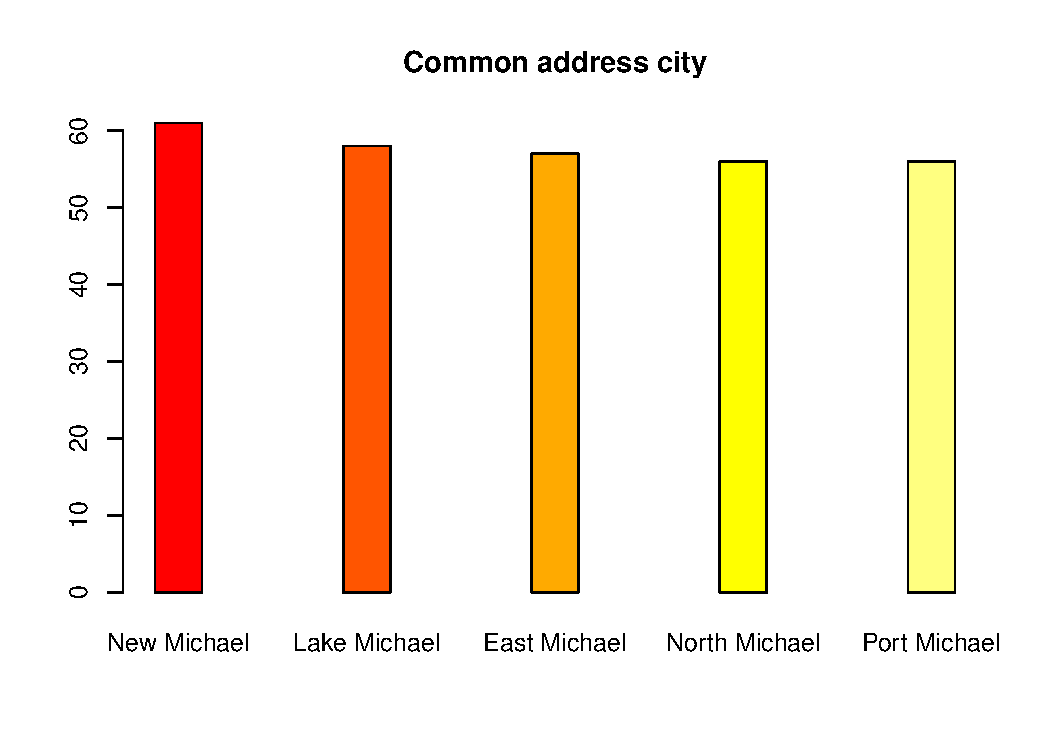
\includegraphics[width=4in]{address_city.pdf}
    \caption{Five most common cities in address.city field. New Michael: 61; Lake Michael: 58; East Michael: 57; North Michael:56; Port Michael: 56}
    \label{fig:address.city}
\end{figure}

\begin{figure}[h]
    \centering
    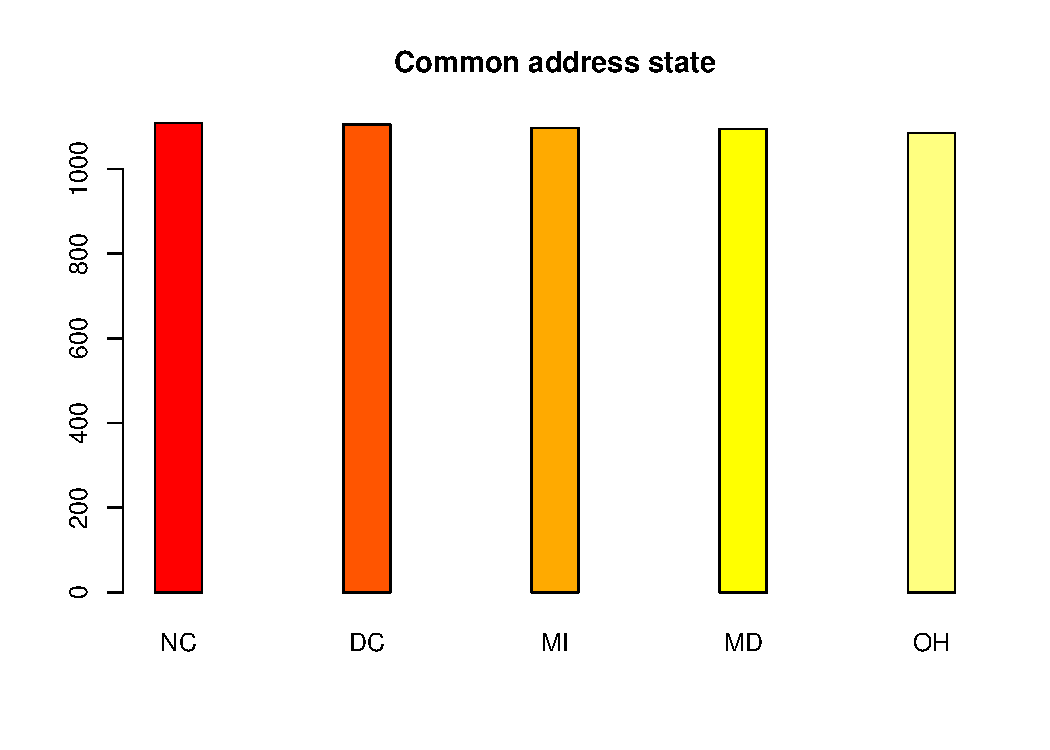
\includegraphics[width=4in]{address_state.pdf}
    \caption{Five most common states in address.city field. NC: 1109; DC: 1106; MI: 1097; MD: 1095; OH: 1085}
    \label{fig:address.state}
\end{figure}

\begin{figure}[h]
    \centering
    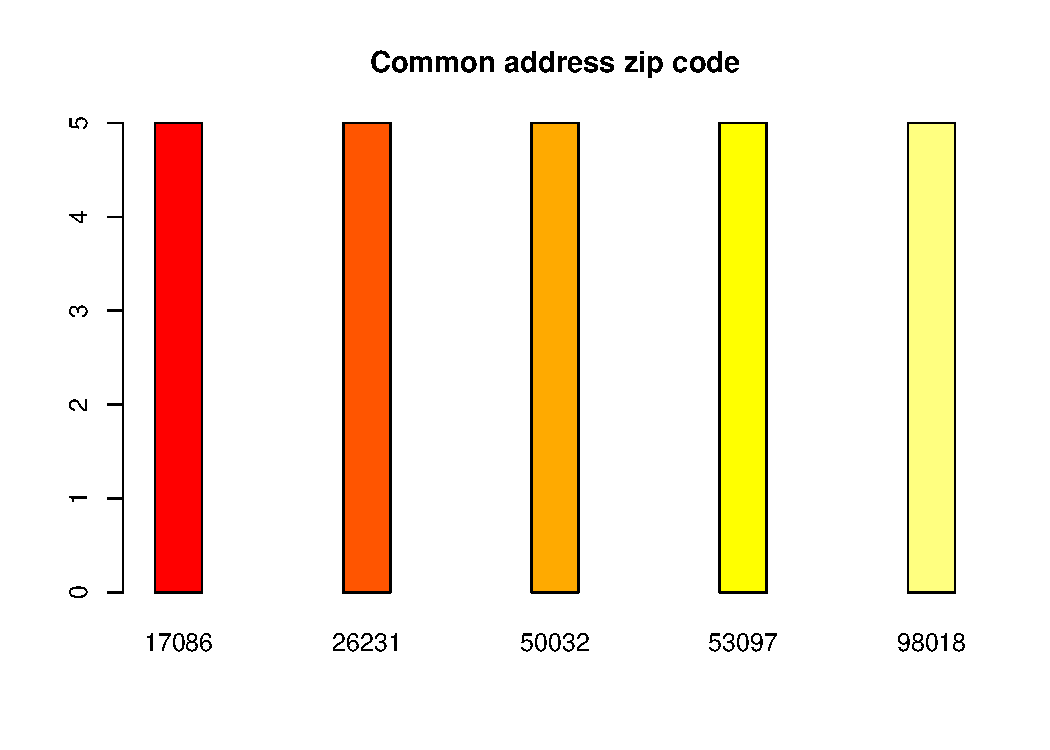
\includegraphics[width=4in]{address_zip.pdf}
    \caption{Five most common zip codes in address.city field. Each common zip code appeared five times.}
    \label{fig:address.zip}
\end{figure}

\begin{figure}[h]
    \centering
    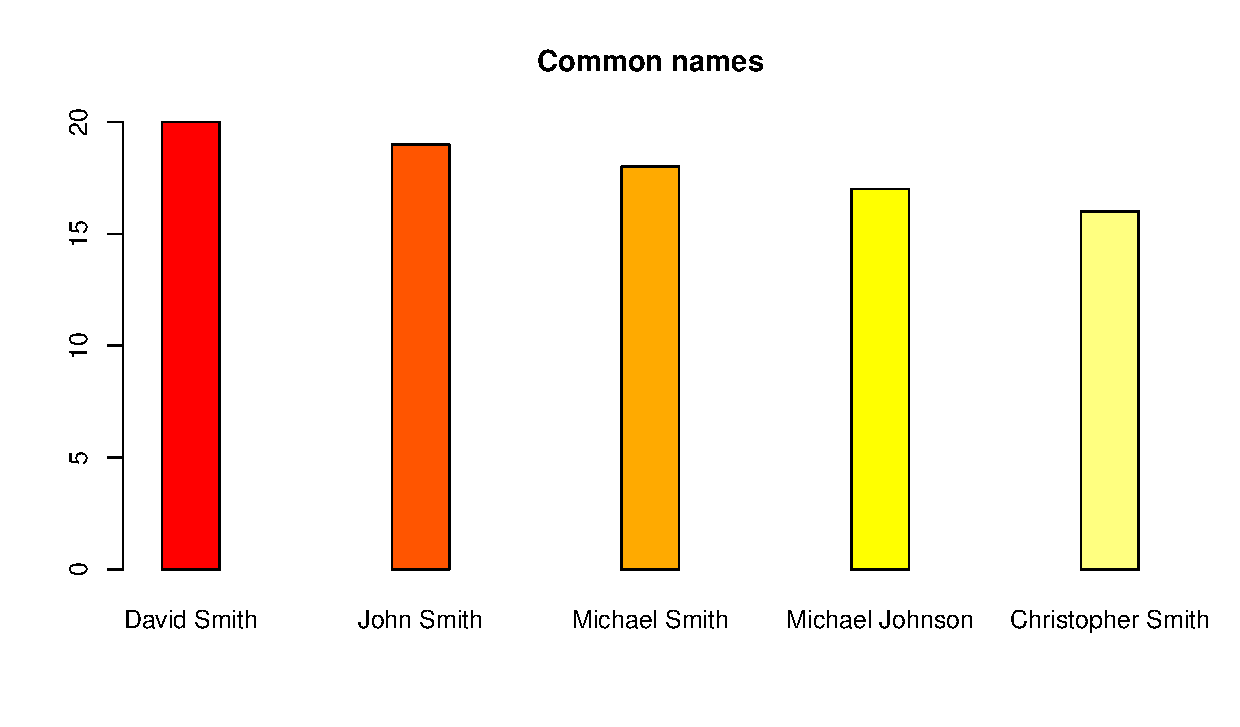
\includegraphics[width=4in]{names.pdf}
    \caption{Five most common names in name field.}
    \label{fig:names}
\end{figure}

\begin{figure}[h]
    \centering
    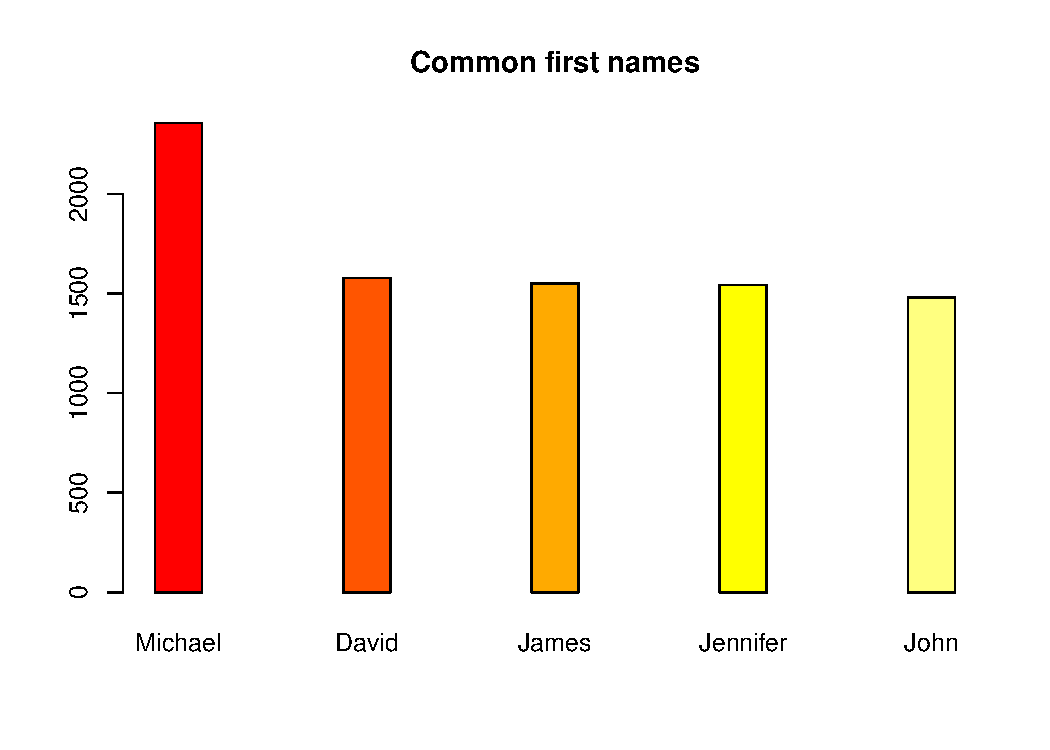
\includegraphics[width=4in]{names_first.pdf}
    \caption{Five most common names in name.first field.}
    \label{fig:names.first}
\end{figure}

\begin{figure}[h]
    \centering
    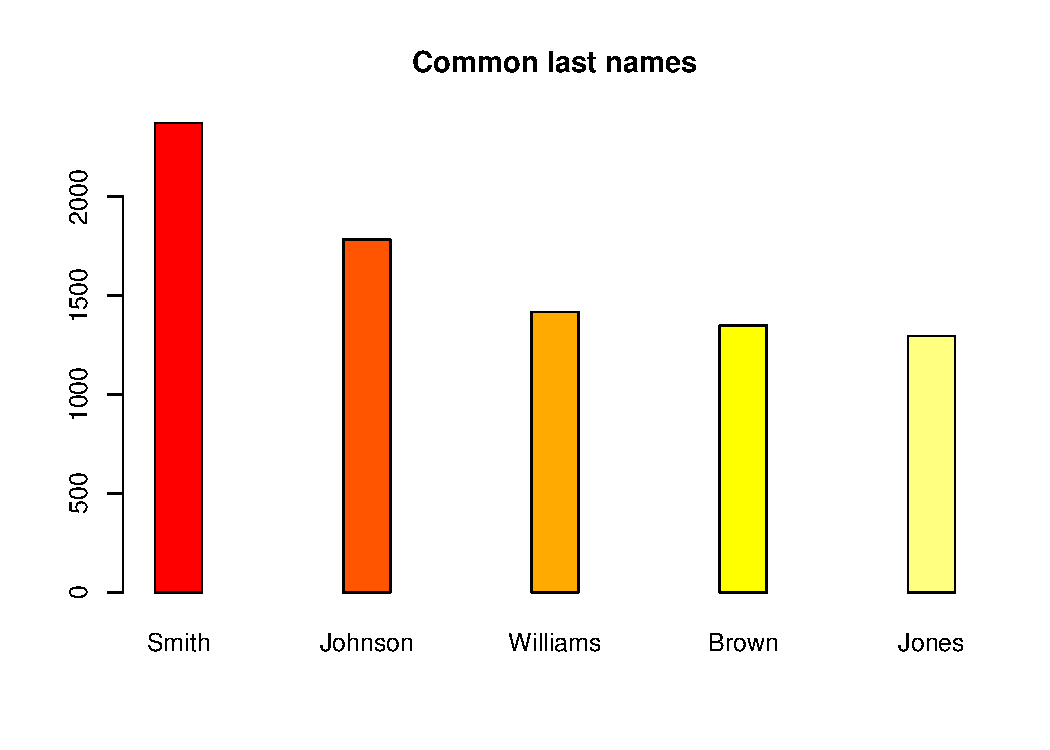
\includegraphics[width=4in]{name_last.pdf}
    \caption{Five most common names in name.last field.}
    \label{fig:names.last}
\end{figure}

\begin{figure}[h]
    \centering
    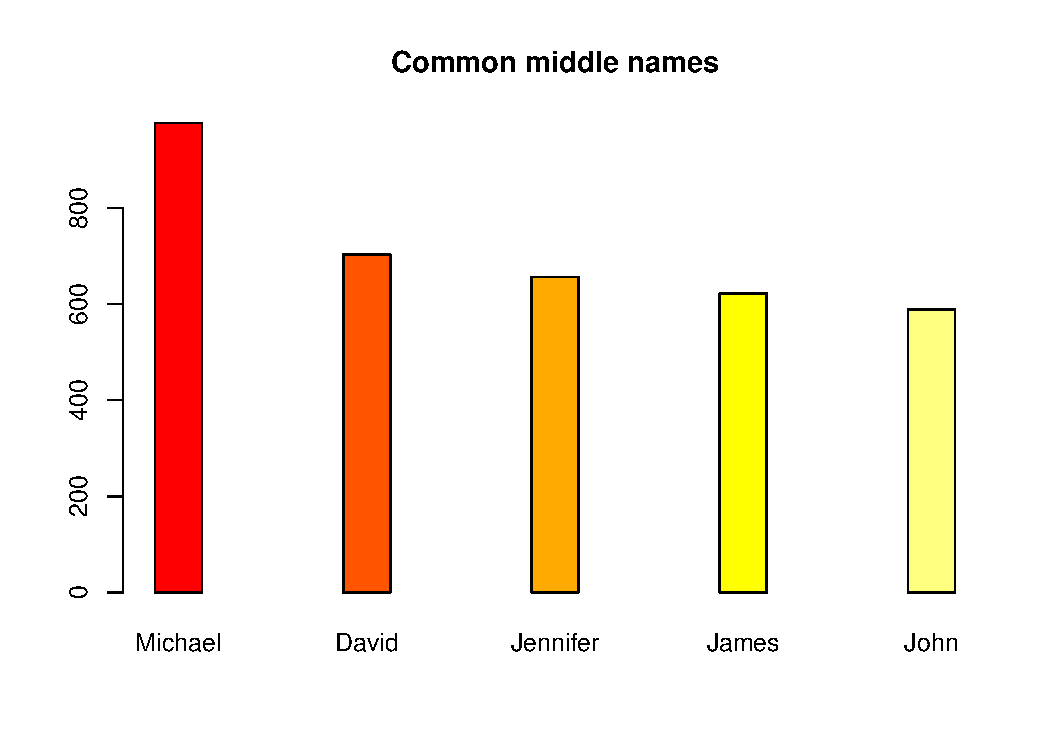
\includegraphics[width=4in]{names_middle.pdf}
    \caption{Five most common names in name.middle field.}
    \label{fig:names.middle}
\end{figure}

The following code was repeated for each field 
\begin{remark}
Field: address.city
    \begin{itemize}
    	\item ac <- sort(table(large\_data\$address.city),decreasing=TRUE)[1:5]
    	\item barplot(ac, main = "Common address city", space=3,col=heat.colors(5))

    \end{itemize}
\end{remark}


%----------------------------------------------------------------------------------------
%	CHAPTER 3
%----------------------------------------------------------------------------------------

%\chapterimage{boat.png}
\chapter{Unique names}

\section{How many distinct first names appear in this data set?}\label{unique_names}

To determine the number of unique first names I looked in the name.first column. From that column, I excluded any NA values, which made up the majority of unique values. Then the unique() function was used to process all unique names. Finally, the length() function yielded the total number of unique names. 

\begin{quote}
\textbf{	"Number of unique first names: 690"}
\end{quote}

\begin{remark}
How many unique first names in small set, excluding NA values    \begin{itemize}
    	\item paste("Number of unique first names:", length(unique(na.exclude(large\_data\$name.first))))
    \end{itemize}
\end{remark}


%----------------------------------------------------------------------------------------
%	CHAPTER 4
%----------------------------------------------------------------------------------------

%\chapterimage{head1.png} % Chapter heading image

\chapter{Unique street names}
\section{How many unique street names?}

To find the number of unique street names I looked in the address.street field. Within that field, the street numbers were stripped using strsplit(), row by row. The results were bound to another data frame with two fields: Street Number and Street Name. 

Once street names were isolated, the unique() function was executed on the column, as used in \ref{unique_names}. I suspect there is a more efficient method of isolating strings. Additionally, with more time I would have included the general address field. Therefore this isn't a complete list of street names, only street names from the address.street column. 

\begin{quote}
	\textbf{"Unique street names: 56858"}
\end{quote}

\begin{figure}[h]
    \centering
    \includegraphics[width=4in]{street_names.pdf}
    \caption{Five most common street names}
    \label{fig:street_names}
\end{figure}

\begin{remark}
# Strips numbers from address.street 
 \begin{itemize}
    	\item street\_names <- lapply(strsplit(large\_data\$address.street, "(?<=\\d)\\b ", perl=T), function(x) if (length(x)<2) c("", x) else x)
    	\item street\_names <- do.call(rbind, street\_names)
    	\item colnames(street\_names) <- c("Street Number", "Street Name")
    \end{itemize}
\end{remark}

\begin{remark}
Find Unique names in street\_names, excluding NA
 \begin{itemize}
    	\item street\_names<- data.frame(street\_names)
    	\item street\_names <- data.frame(lapply(street\_names, as.character), stringsAsFactors=FALSE)
    	\item paste("Unique street names:",length(unique(na.exclude(street\_names\$Street.Name))))
    	\item barplot(sort(table(street\_names\$Street.Name),decreasing=TRUE)[1:5], main = "Five most common street names", space=3, col=heat.colors(5) )
    \end{itemize}
\end{remark}

%----------------------------------------------------------------------------------------
%	CHAPTER 5
%----------------------------------------------------------------------------------------

%\chapterimage{head1.png} % Chapter heading image

\chapter{Five most common area codes}

To find the five most common area codes in the phone number field I began by stripping all special characters. The special characters were stripped with the gsub() function. Then I attempted to strip the "1 " in front of some of the numbers, again with gsub(). Invoking gsub() again I removed all whitespace. Finally, with substring(), I isolated the first three numbers, presumably the area code. As a first time user of R, stripping strings is definitely an area for improvement. Regardless, the results are plotted below: 

\begin{figure}[h]
    \centering
    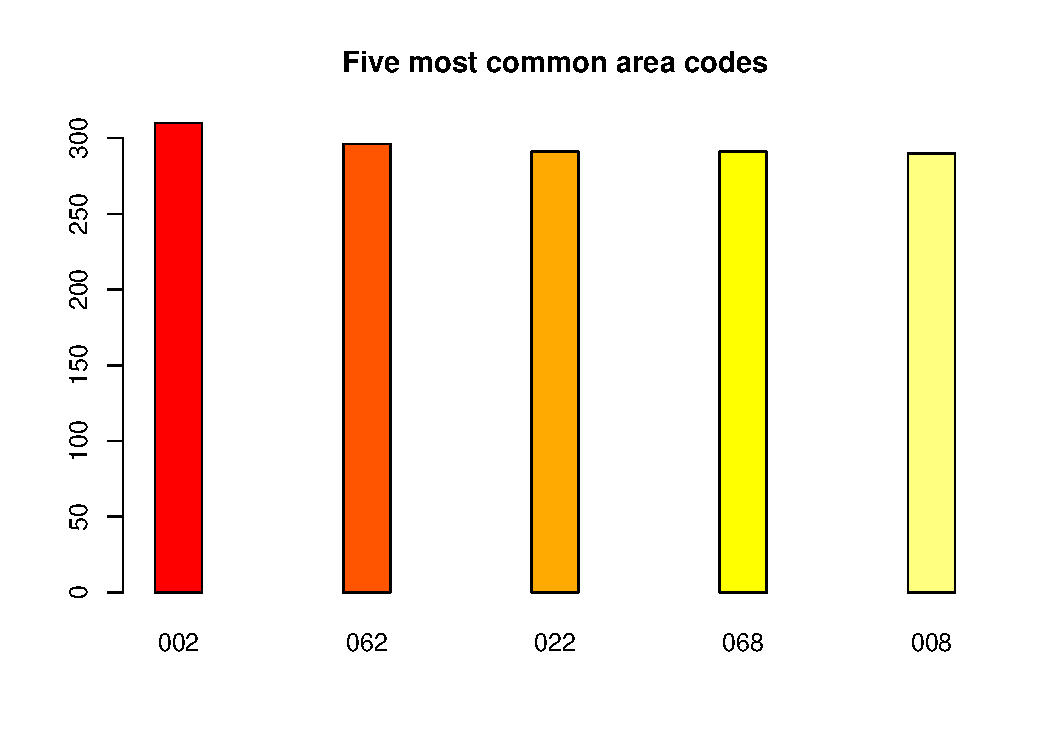
\includegraphics[width=4in]{five_area_codes.pdf}
    \caption{Five most common area codes}
    \label{fig:common_codes}
\end{figure}

\begin{remark}
Approach for finding US area codes
 \begin{itemize}
    	\item area\_codes <- large\_data\$phone
    	\item area\_codes <- gsub("[[:punct:]]", " ", area\_codes)
    	\item area\_codes <- gsub("1 ", " ", area\_codes)
    	\item area\_codes <- gsub(" ", "", area\_codes, fixed = TRUE)
    	\item area\_codes <- substring(area\_codes, 1, 3)
    	\item barplot(sort(table(area\_codes),decreasing=TRUE)[1:5], main = "Five most common area codes", space=3, col=heat.colors(5) )
    \end{itemize}
\end{remark}

\end{document}